% !TeX spellcheck = en_US
%\documentclass[11pt,a4paper]{article}
\documentclass[11pt
  , a4paper
  , article
  , oneside
%  , twoside
%  , draft
]{memoir}

\usepackage{control}
\usepackage[numbers]{natbib}


\begin{document}

\newcommand{\technumber}{
  RAON Control-Document Series\\
  Revision : v1.0,   Release : 2015-03-16 fixed date}
\title{\textbf{Vivado를 사용한 FPGA Logic Gate Simulation}}

\author{이상일\thanks{silee7103@ibs.re.kr}, 손창욱 \\

  Rare Isotope Science Project\\
  Institute for Basic Science, Daejeon, South Korea
}
\date{\today}
\renewcommand{\maketitlehooka}{\begin{flushright}\textsf{\technumber}\end{flushright}}
%\renewcommand{\maketitlehookb}{\centering\textsf{\subtitle}}
%\renewcommand{\maketitlehookc}{C}
%\renewcommand{\maketitlehookd}{D}

\maketitle

\begin{abstract}
FPGA 개발의 초석이 되는 Digital Logic Gate 설계는 VerilogHDL(Hardware Description Language) 언어를 이용한다. Vivado를 이용하여 VerilogHDL 코드를 사용한 모듈 설계 방법 및 그에 대한 Test Bench Code를 작성하여 Simulation 하는 기본적인 흐름을 기술한다.
\end{abstract}

\chapter{Vivado - Project 생성}
 본 문서에서는 JK-FlipFlop에 대한 Logic module을 설계 후 그에 대한 Test Bench Code를 작성하여 Simulation 한다. File 메뉴->New Project...를 선택하면 그림 \ref{fig:vivado_1}과 같은 화면이 생성된다. Next 화면으로 이동 후 그림 \ref{fig:vivado_2}와 같이 "Project Name" 및 "Project location"을 지정한다.

\clearpage

\begin{figure}[h!]
	\centering
	\includegraphics[width=0.8\textwidth, height=0.4\textwidth]{./images/vivado-pro-1.eps}
	\caption{Vivado Project 생성}
	\label{fig:vivado_1} 
\end{figure}


\begin{figure}[h!]
	\centering
	\includegraphics[width=0.8\textwidth, height=0.4\textwidth]{./images/vivado-pro-2.eps}
	\caption{Project Name 및 location}
	\label{fig:vivado_2} 
\end{figure}

Next 화면으로 이동 후 "Project Type"에서 RTL Project를 선택 후 Next 화면으로 이동한다. [그림\ref{fig:vivado_3}]
Target language "Verilog", Simulator language "Mixed" 디폴트 설정을 확인 후 "Create File..." 버튼을 눌러 File name "jkflipflop"을 입력한다. Next 화면 "Add Existing IP(optional)"은 Project에 포함 될 Existing IP를 추가하는 내용이다. 현재는 추가 없이 Next 화면으로 이동, "Add Constraints(optional)" 화면 역시 추가 구성 없이 Next 화면으로 이동한다. 그림 \ref{fig:vivado_4}에서와 같의 Default Part 부분에서 "Boards" 버튼 -> "Display Name"에서 "ZedBoard Zynq Evaluation and Development Kit"을 선택 한 후 해당 보드를 선택한 후 Next -> Finish를 클릭한다.

\hfil\break

\begin{figure}[h!]
	\centering
	\includegraphics[width=0.8\textwidth, height=0.4\textwidth]{./images/vivado-pro-3.eps}
	\caption{Create Source File}
	\label{fig:vivado_3} 
\end{figure}	

\begin{figure}[h!]
	\centering
	\includegraphics[width=0.8\textwidth, height=0.4\textwidth]{./images/vivado-pro-4.eps}
	\caption{개발 보드 선택}
	\label{fig:vivado_4} 
\end{figure}	

\clearpage

그림 \ref{fig:vivado_5}는 HDL module의 입/출력을 정의하는 화면이다. 그림에서와 같이 입/출력을 정의한다. 입/출력 구성이 완료되면 그림\ref{fig:vivado_6}와 같은 모듈 구성 입력 창이 생성된다.

\begin{figure}[h!]
	\centering
	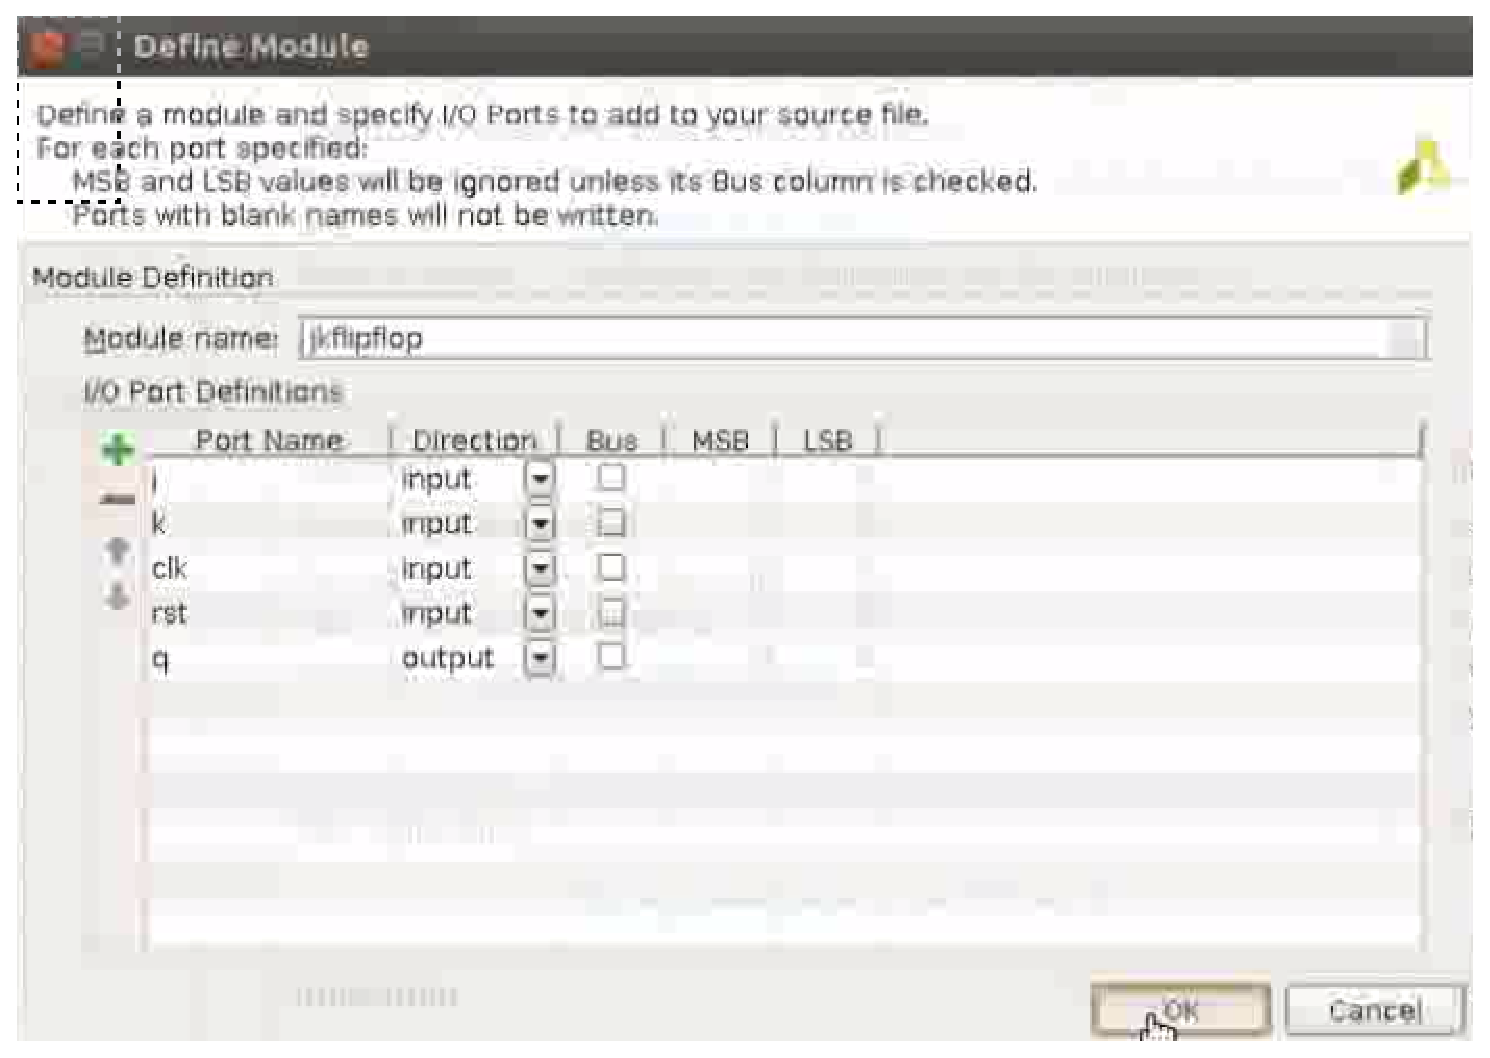
\includegraphics[width=0.8\textwidth, height=0.4\textwidth]{./images/vivado-pro-5.eps}
	\caption{Module 입출력 정의}
	\label{fig:vivado_5} 
\end{figure}	

\begin{figure}[h!]
	\centering
	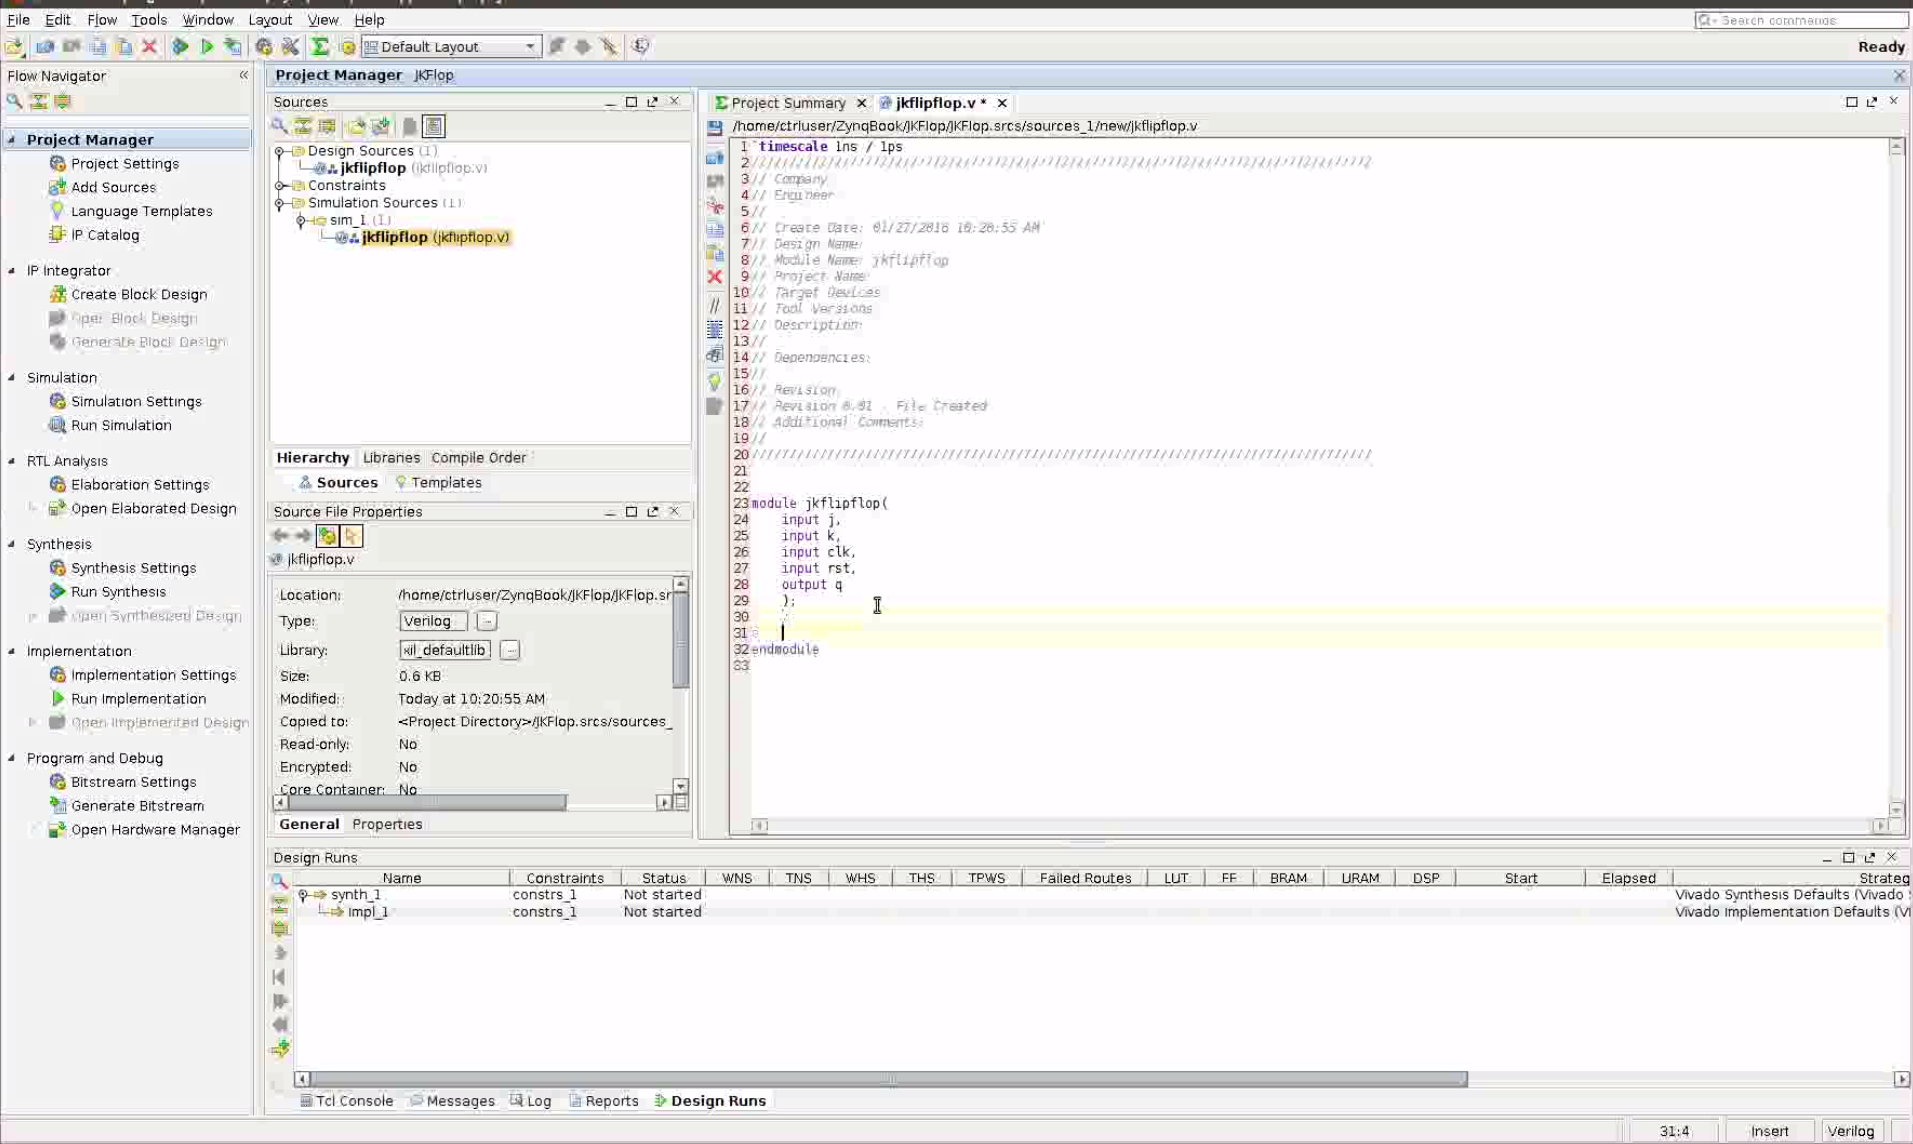
\includegraphics[width=0.8\textwidth, height=0.4\textwidth]{./images/vivado-pro-6.eps}
	\caption{모듈 구성 입력 창}
	\label{fig:vivado_6} 
\end{figure}	

모듈 구성 입력 창을 통해 아래 그림 \ref{fig:vivado_7}과 같은 verilogHDL 코드를 작성한다.

\begin{figure}[h!]
	\centering
	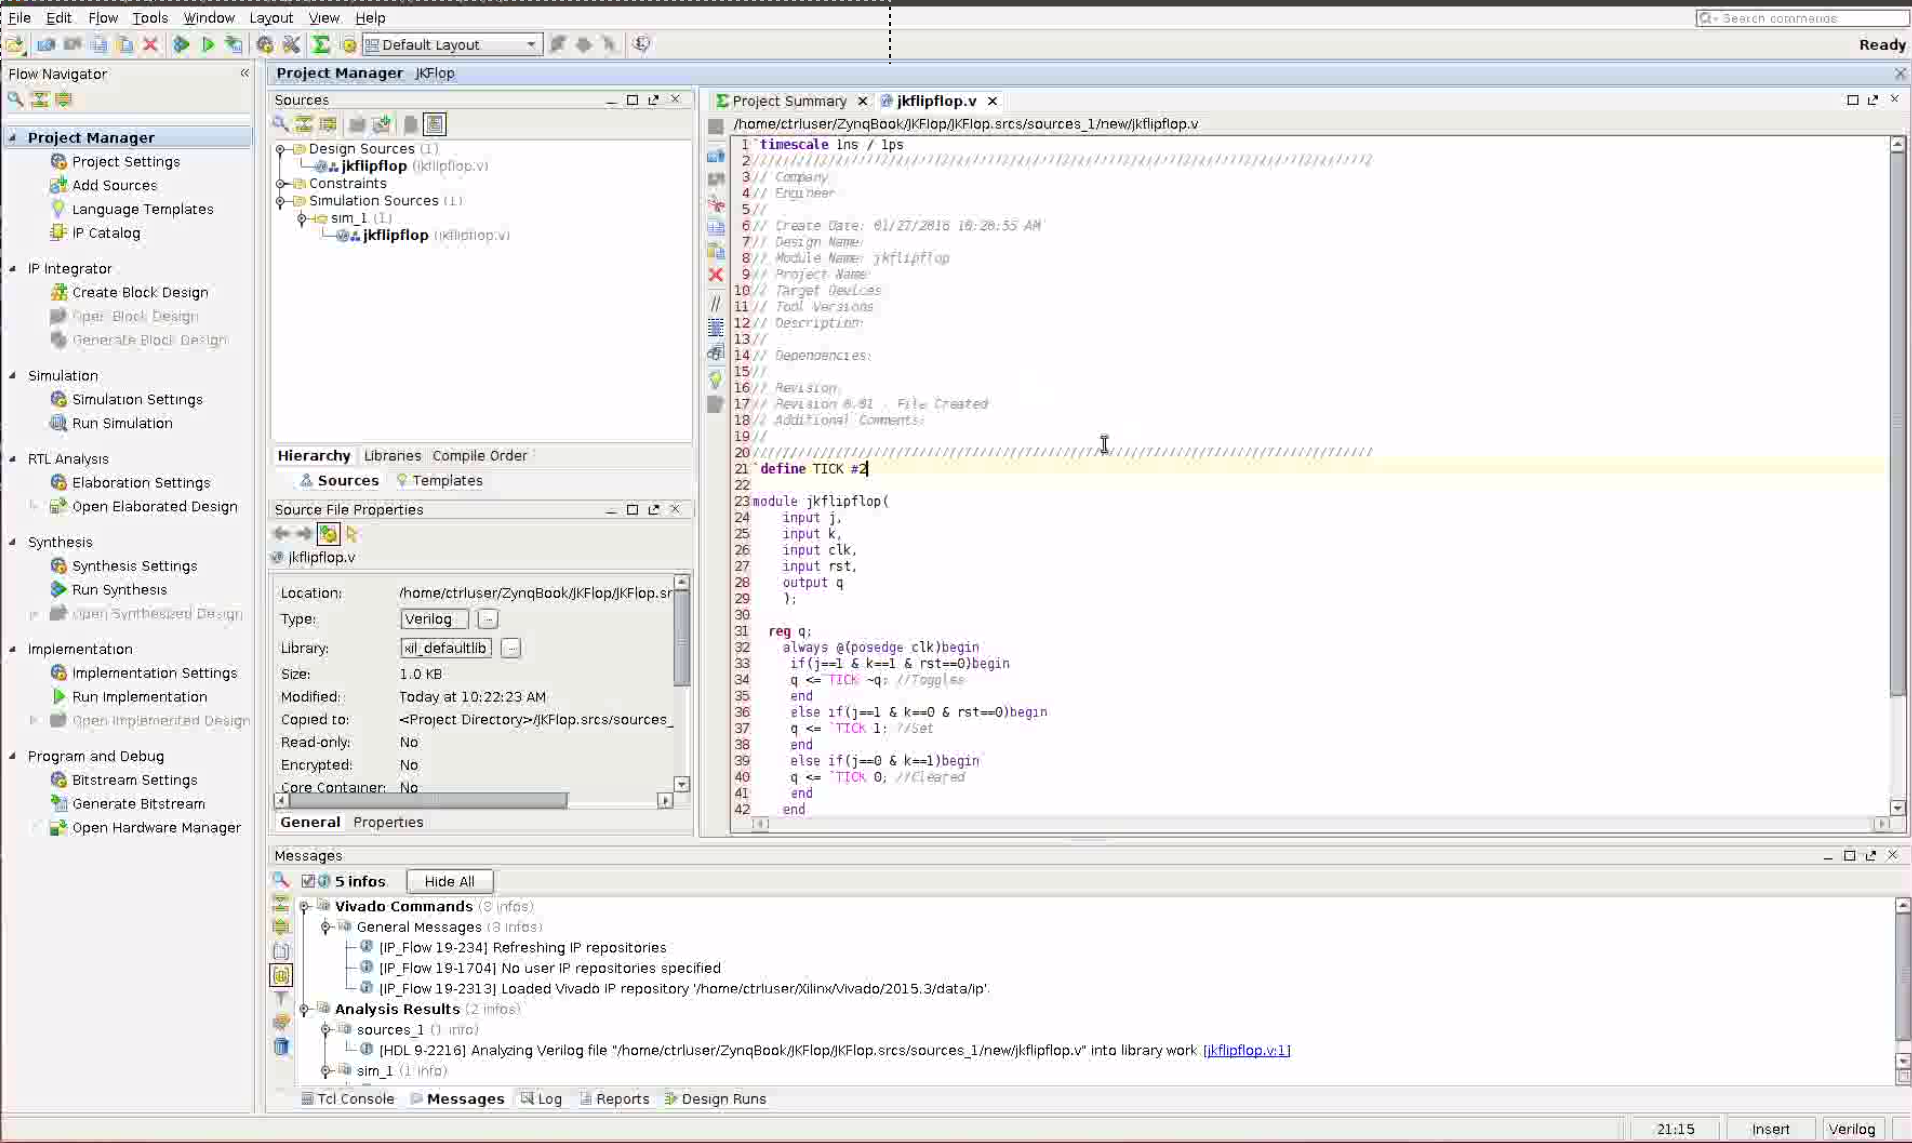
\includegraphics[width=1.1\textwidth, height=0.8\textwidth]{./images/vivado-pro-7.eps}
	\caption{Delay 정의}
	\label{fig:vivado_7} 
\end{figure}
	
\clearpage

\begin{lstlisting}[style=termstyle, escapechar=!]
!\color{codegreen}{
`timescale 1ns / 1ps \
////////////////////////////////////////////////////////////////////////////////// \\
// Company: \\
// Engineer: \\
// \\
// Create Date: 01/27/2016 10:20:55 AM \\
// Design Name: \\
// Module Name: jkflipflop \\
// Project Name: \\
// Target Devices: \\ 
// Tool Versions: \\
// Description: \\
// Dependencies: \\
// \\
// Revision: \\
// Revision 0.01 - File Created \\
// Additional Comments: \\
////////////////////////////////////////////////////////////////////////////////// \\

`define TICK \#2 \\
module jkflipflop( \\
input j,\\
input k,\\
input clk,\\
input rst,\\
output q\\
);\\

reg q;\\
always @(posedge clk)begin\\
if(j==1 \& k==1 \& rst==0) begin\\
q <=`TICK ~q; //Toggles\\
end\\
else if(j==1 \& k==0 \& rst==0)begin\\
q <= `TICK 1; //Set\\
end\\
else if(j==0 \& k==1)begin\\
q <= `TICK 0; //Cleared\\
end\\
end\\
always @(posedge rst)begin\\
q <= 0; //The reset normally has negligible delay and hence ignored.\\
end\\
endmodule\\
}! 
\end{lstlisting}

작성된 모듈의 Simulation을 위한 Test Bench Code 추가를 위하여 아래 그림 \ref{fig:vivado_8} 에서 그림 \ref{fig:vivado_12} 까지의 절차를 따라 수행 하며, 그림 \ref{fig:vivado_12}의 코드를 작성한다.

\begin{figure}[h!]
	\centering
	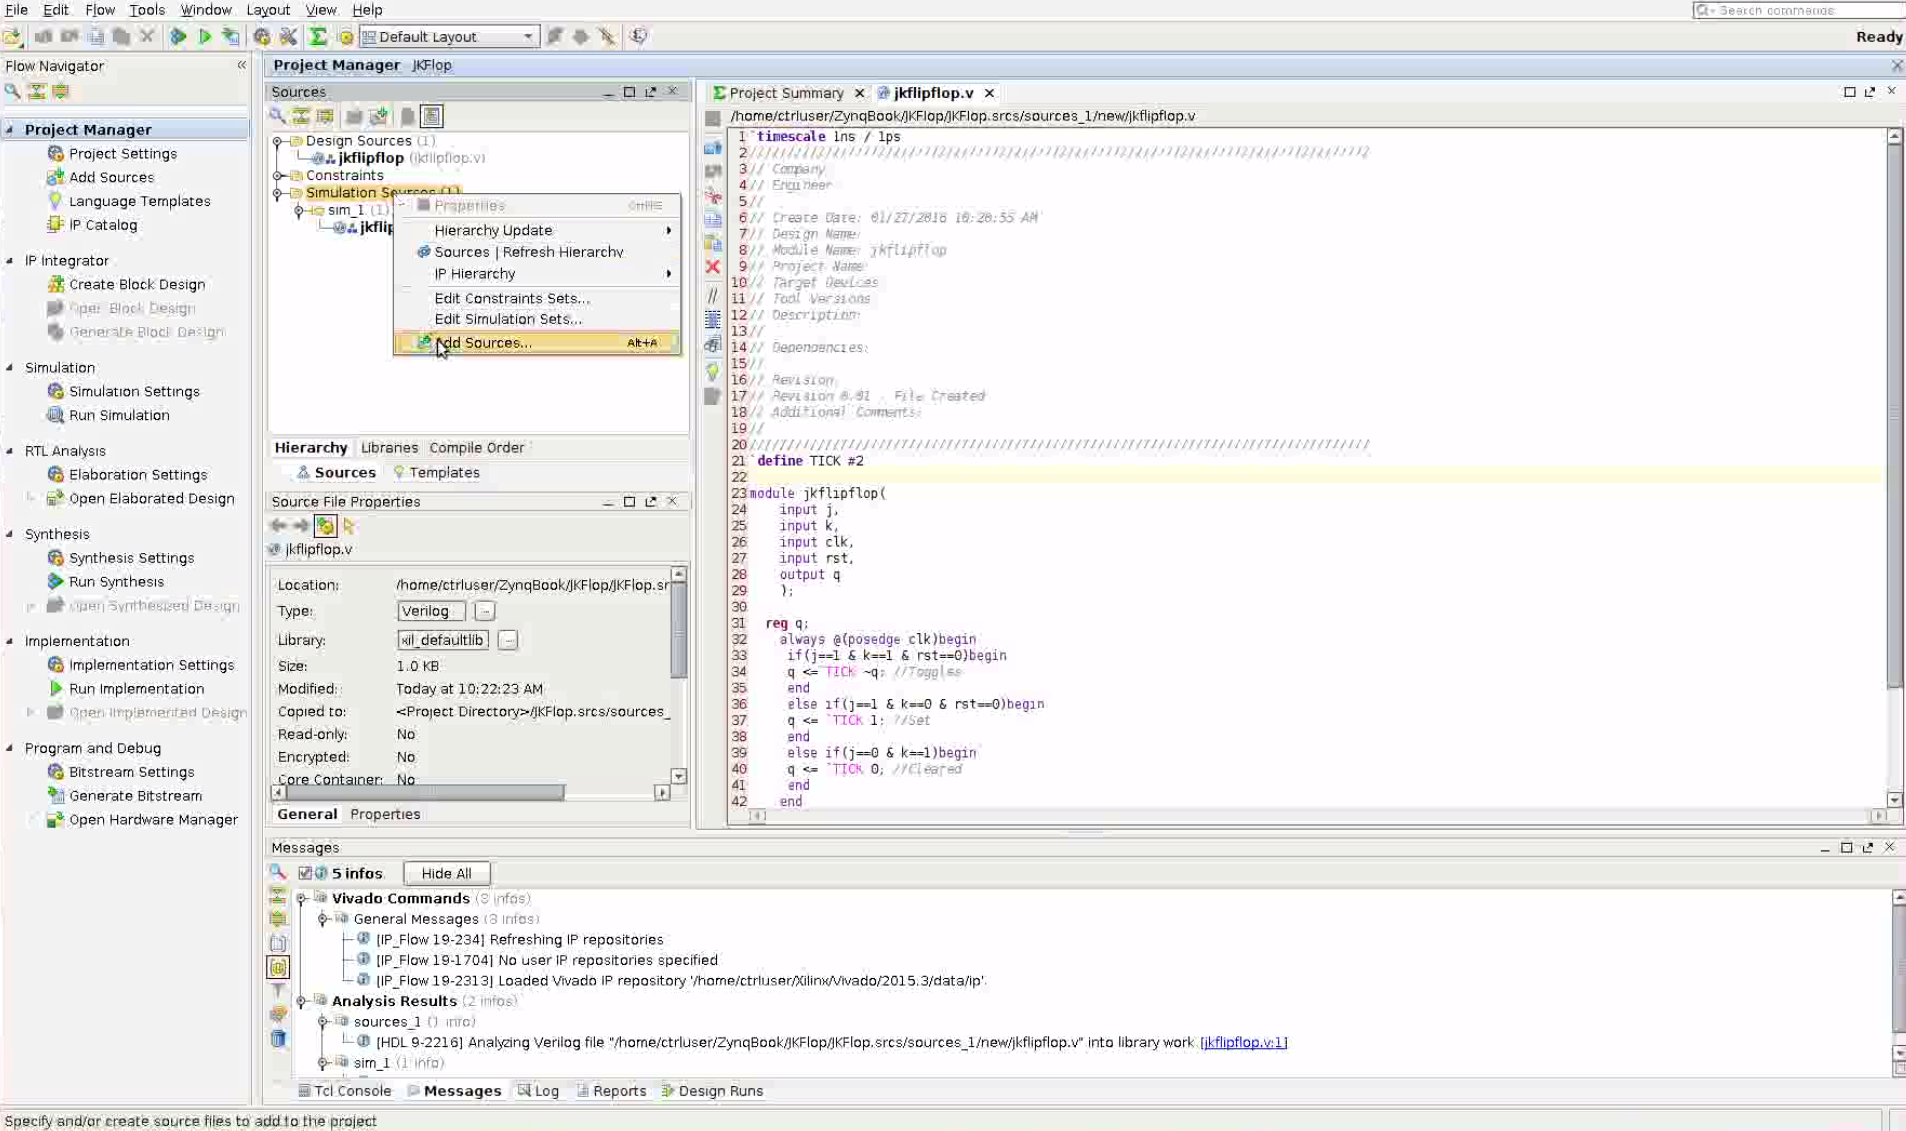
\includegraphics[width=0.8\textwidth, height=0.4\textwidth]{./images/vivado-pro-8.eps}
	\caption{Test Bench Code 추가 1}
	\label{fig:vivado_8} 
\end{figure}	

\begin{figure}[h!]
	\centering
	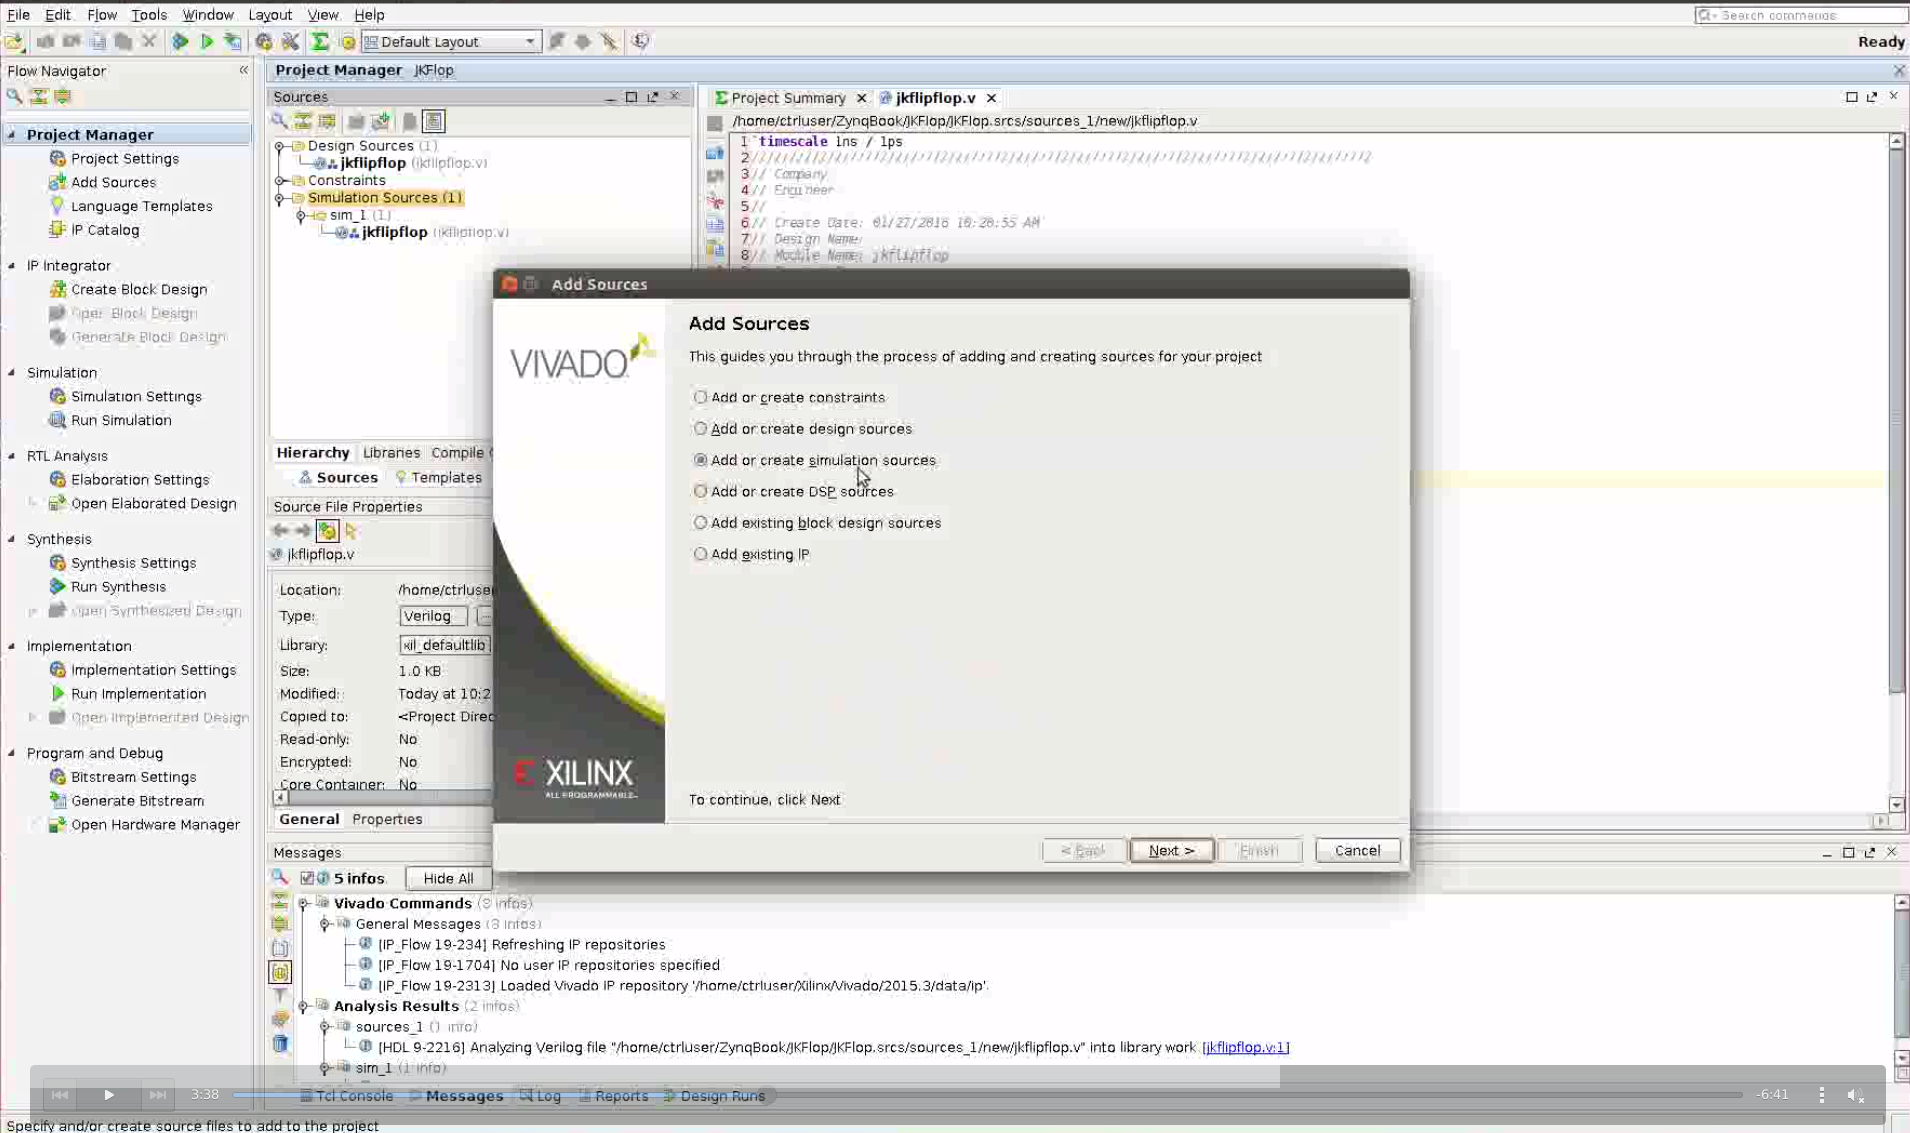
\includegraphics[width=0.8\textwidth, height=0.4\textwidth]{./images/vivado-pro-9.eps}
	\caption{Test Bench Code 추가 2}
	\label{fig:vivado_9} 
\end{figure}	


\begin{figure}[h!]
	\centering
	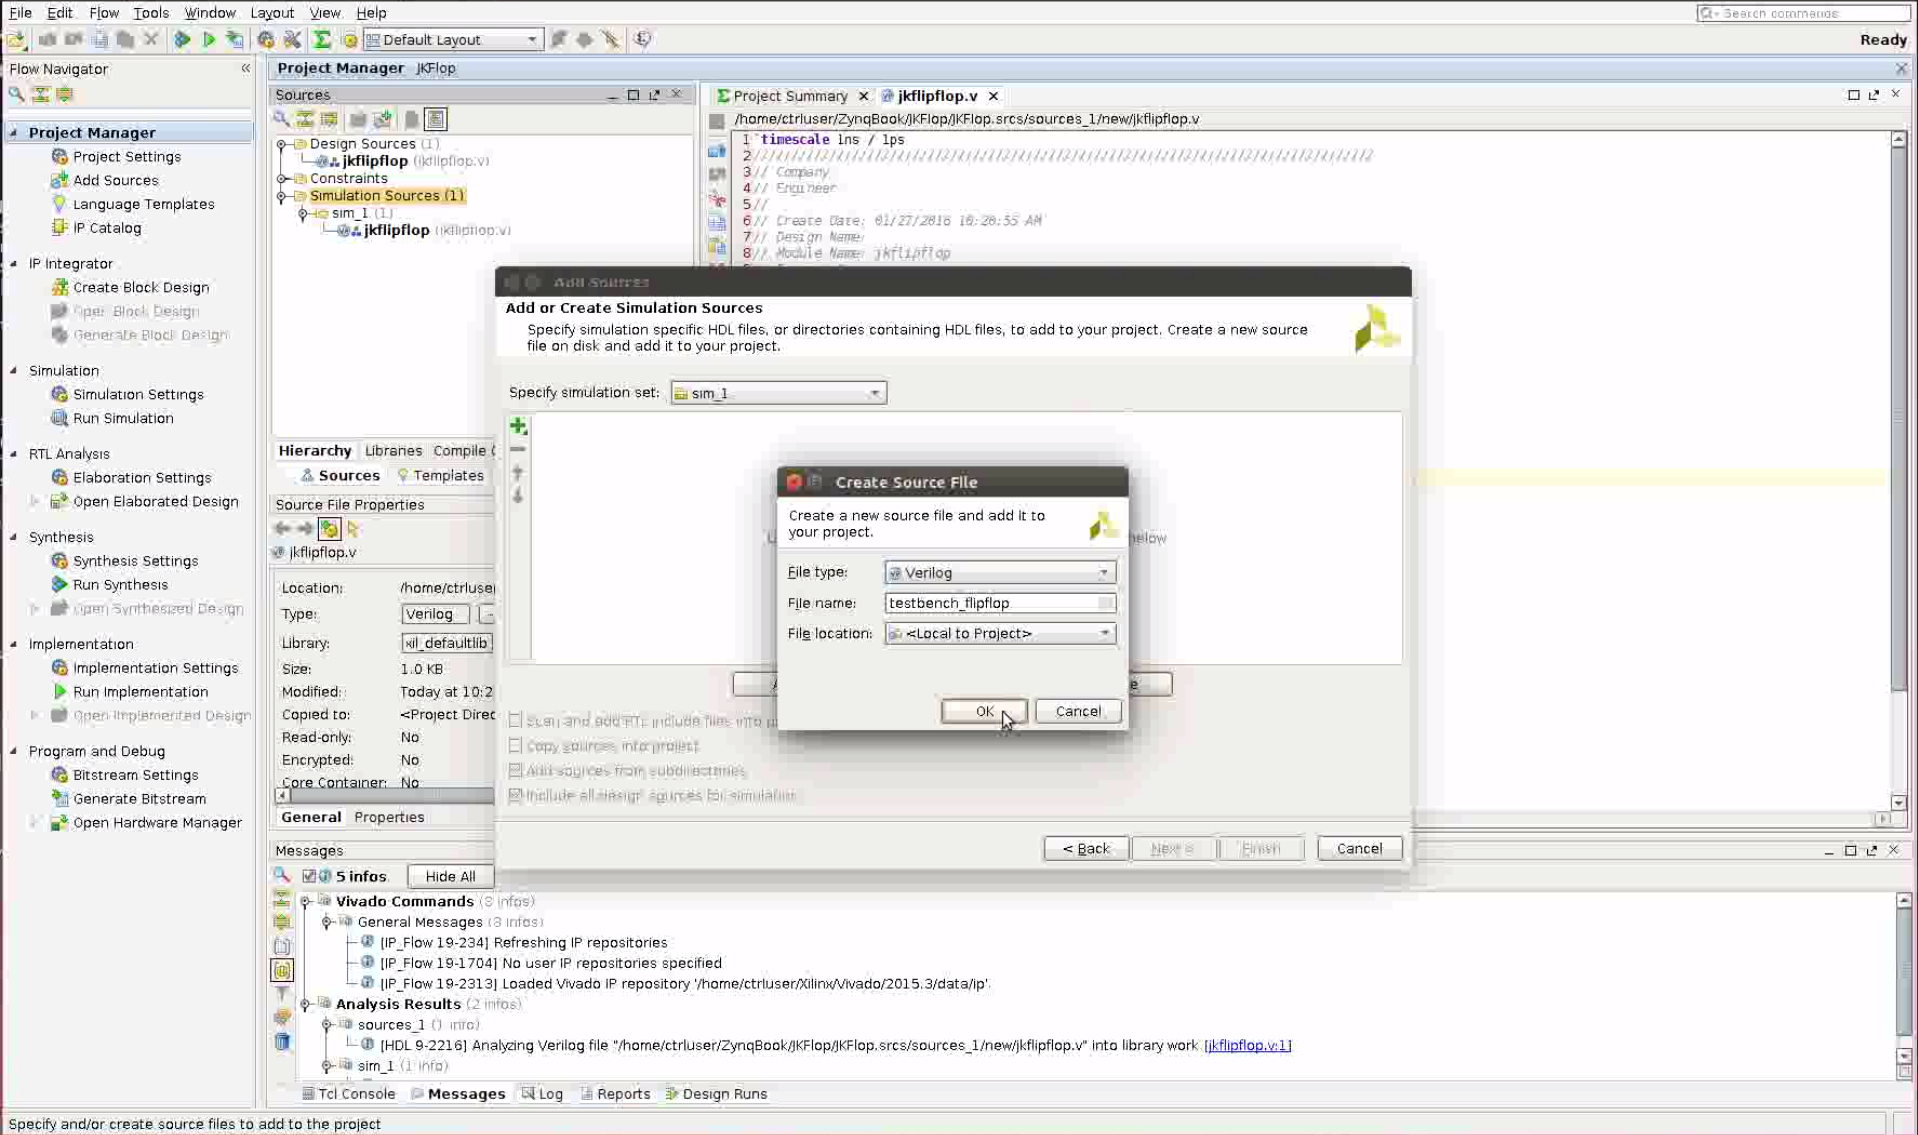
\includegraphics[width=0.8\textwidth, height=0.4\textwidth]{./images/vivado-pro-10.eps}
	\caption{Test Bench Code 추가 3}
	\label{fig:vivado_10} 
\end{figure}	

\begin{figure}[h!]
	\centering
	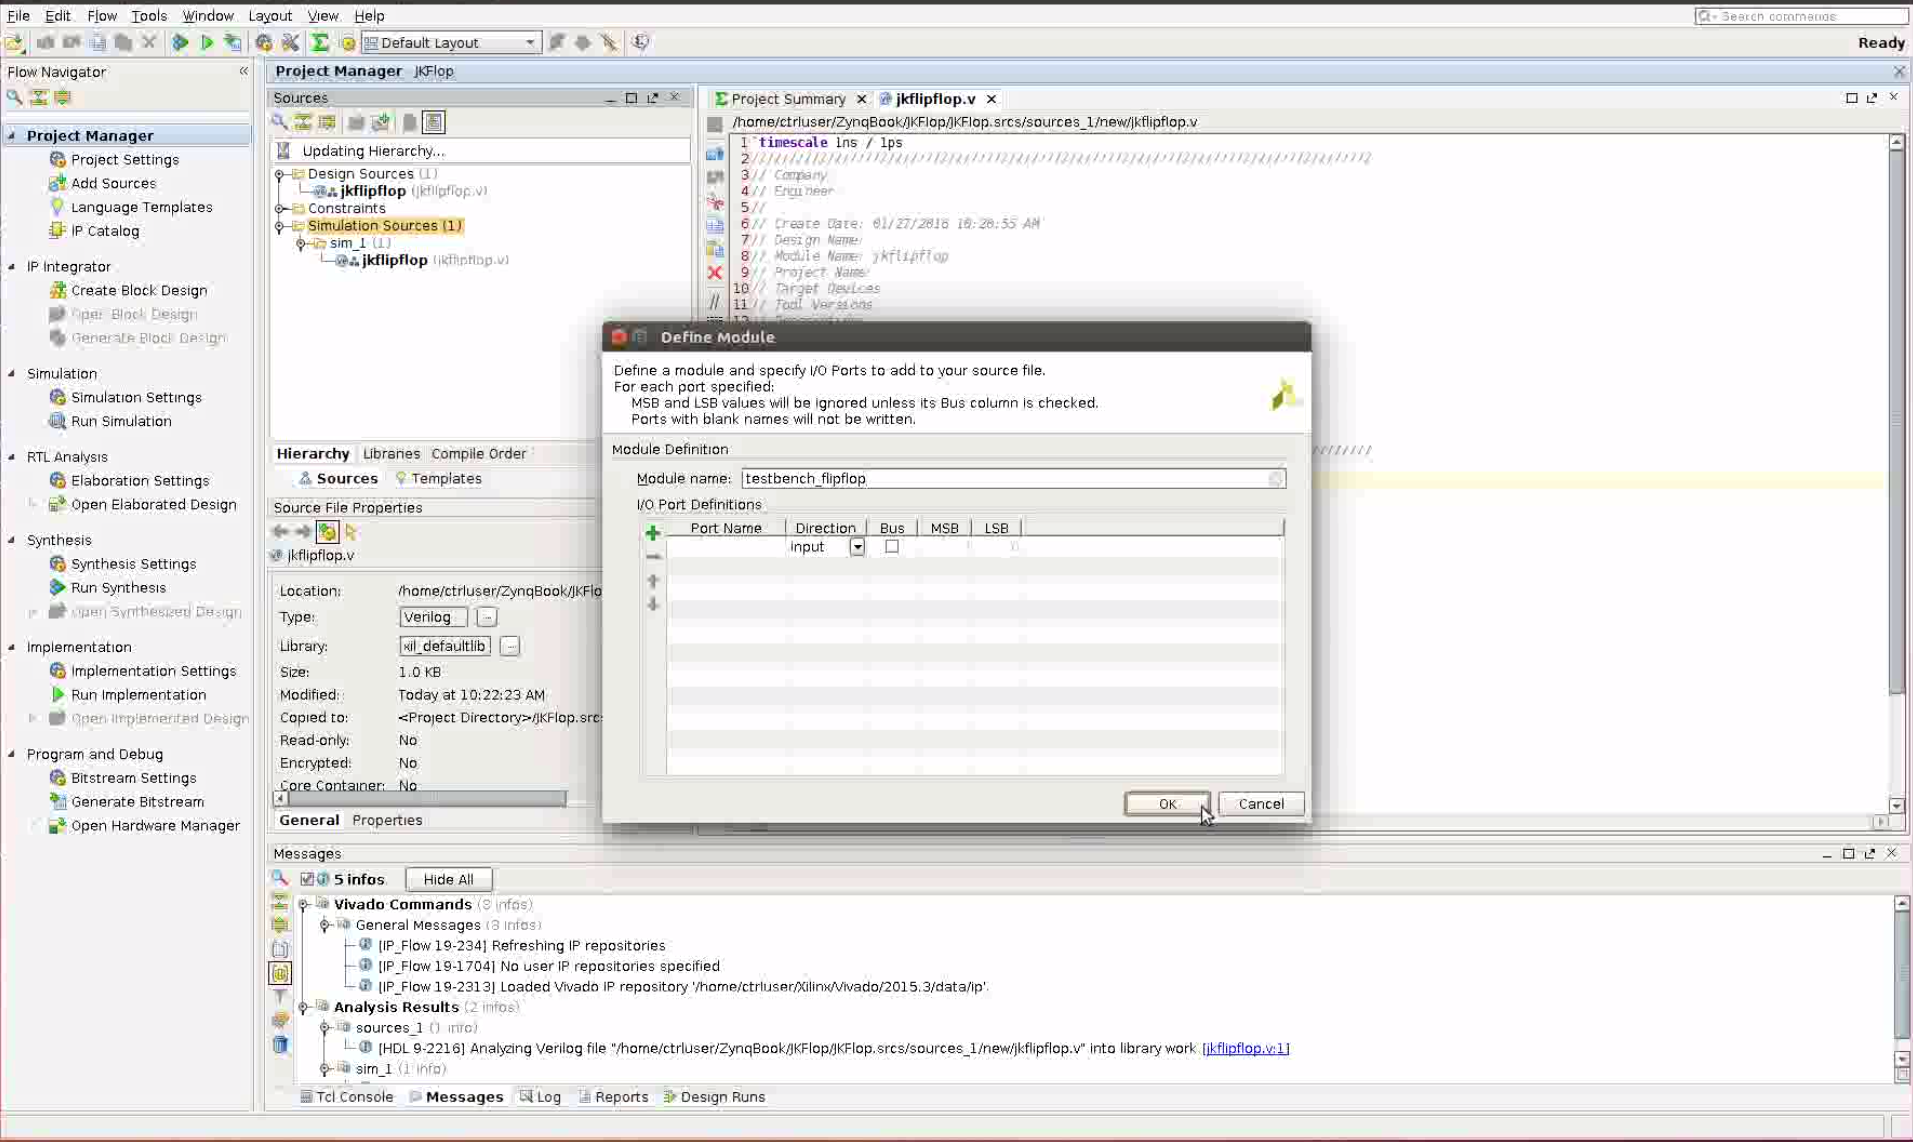
\includegraphics[width=0.8\textwidth, height=0.4\textwidth]{./images/vivado-pro-11.eps}
	\caption{Test Bench Code 추가 4}
	\label{fig:vivado_11} 
\end{figure}

\begin{figure}[h!]
	\centering
	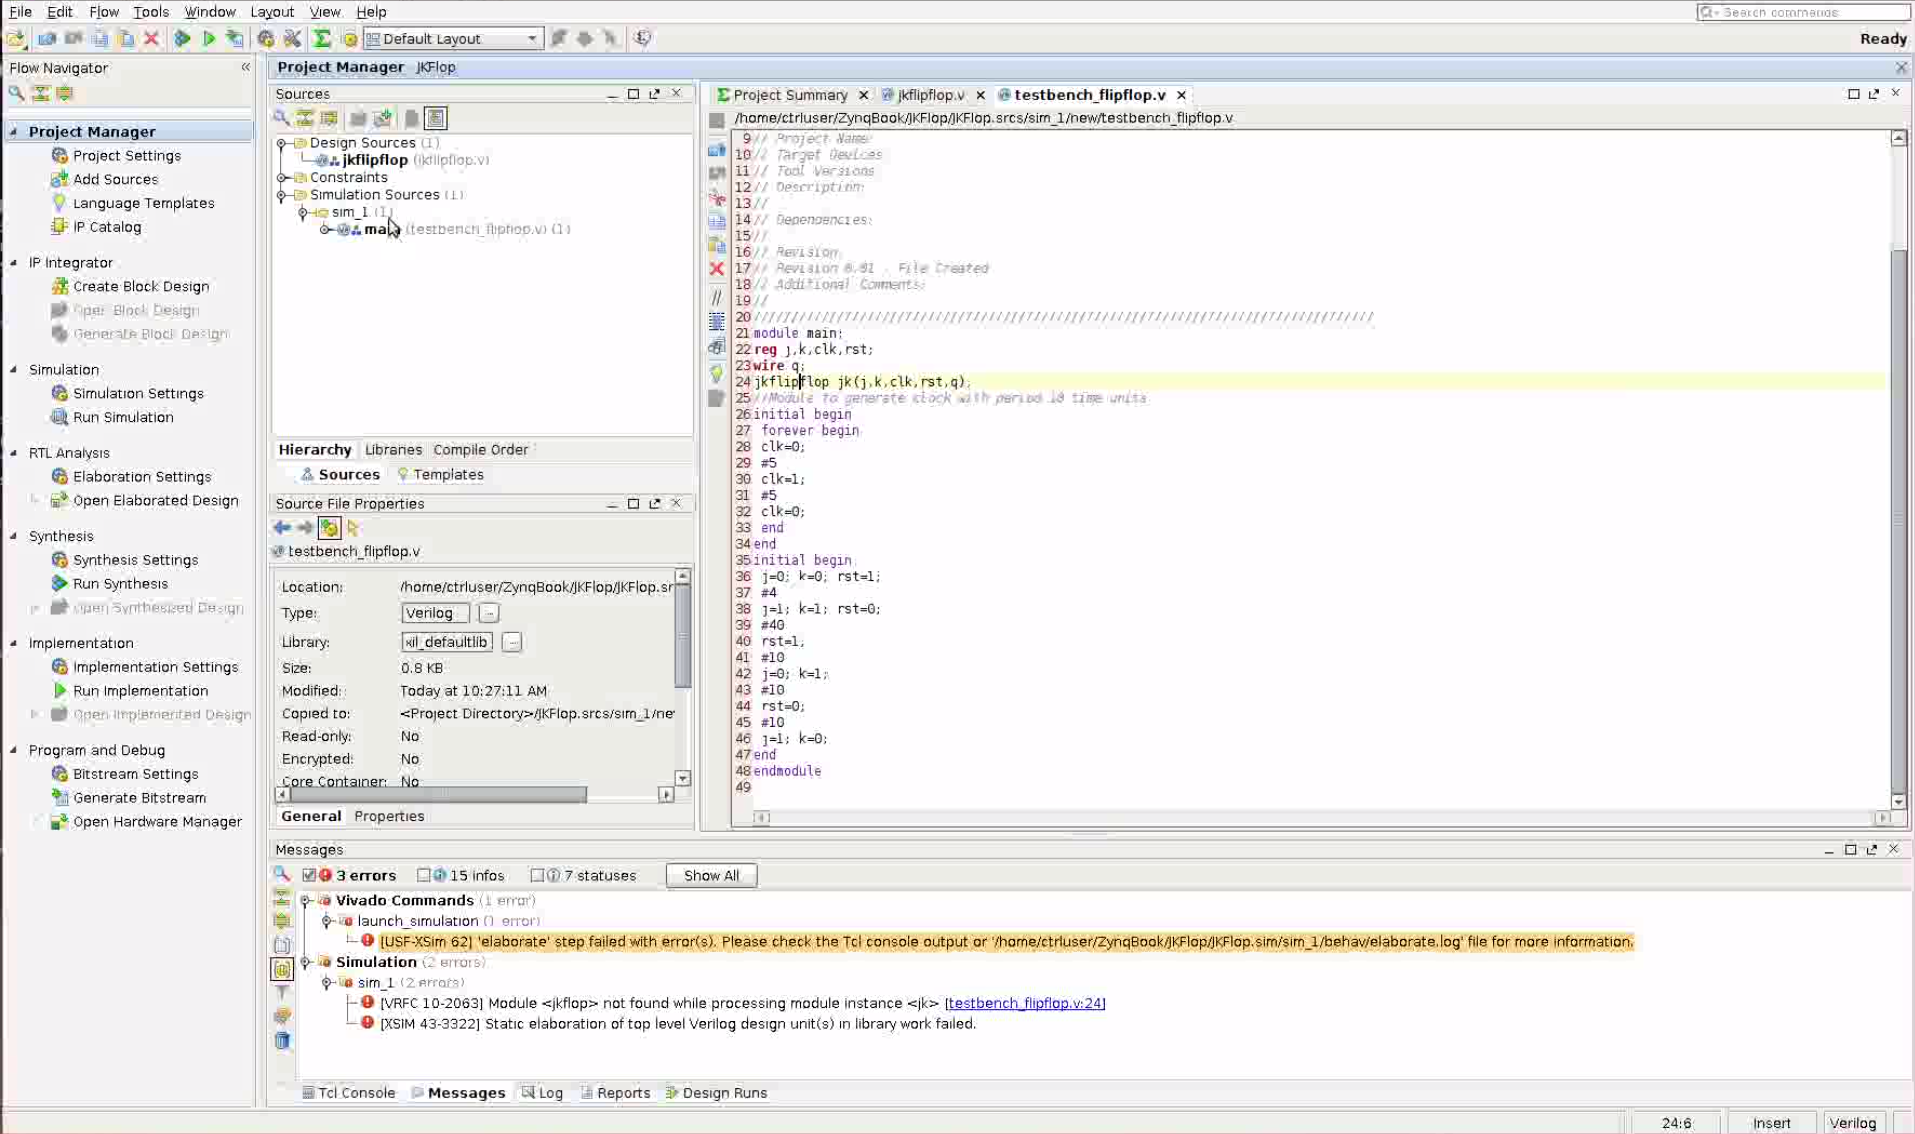
\includegraphics[width=1.1\textwidth, height=0.8\textwidth]{./images/vivado-pro-12.eps}
	\caption{Test Bench Code 추가 5}
	\label{fig:vivado_12} 
\end{figure}
\clearpage
\begin{lstlisting}[style=termstyle, escapechar=!]
!\color{codegreen}{
`timescale 1ns / 1ps \\
//////////////////////////////////////////////////////////////////////////////////\\
// Company: \\
// Engineer: \\
// \\
// Create Date: 01/27/2016 10:23:09 AM\\
// Design Name: \\
// Module Name: testbench\_flipflop\\
// Project Name: \\
// Target Devices: \\
// Tool Versions: \\
// Description: \\
// \\
// Dependencies: \\
// \\
// Revision:\\
// Revision 0.01 - File Created\\
// Additional Comments:\\
// \\
//////////////////////////////////////////////////////////////////////////////////\\
module main;\\
reg j,k,clk,rst;\\
wire q;\\
jkflipflop jk(j,k,clk,rst,q);\\
//Module to generate clock with period 10 time units\\
initial begin\\
forever begin\\
clk=0;\\
\#5\\
clk=1;\\
\#5\\
clk=0;\\
end\\
end\\
initial begin\\
j=0; k=0; rst=1;\\
\#4\\
j=1; k=1; rst=0;\\
\#40\\
rst=1;\\
\#10\\
j=0; k=1;\\
\#10\\
rst=0;\\
\#10\\
j=1; k=0;\\
end\\
endmodule\\

\end{lstlisting}

\clearpage

Test Bench Code의 작성이 완료된 후 Project Manager Window의 Simulation 항목의 "Simulation Setup"을 구성후 "Run Simulation"을
실행한다. Simulation의 완료된 후 그림 \ref{fig:sim_1} 에서 그림 \ref{fig:sim_6}까지 해당 모듈의 Logic에 대한 Simulation이 이상없는지 확인한다.

\begin{figure}[h!]
	\centering
	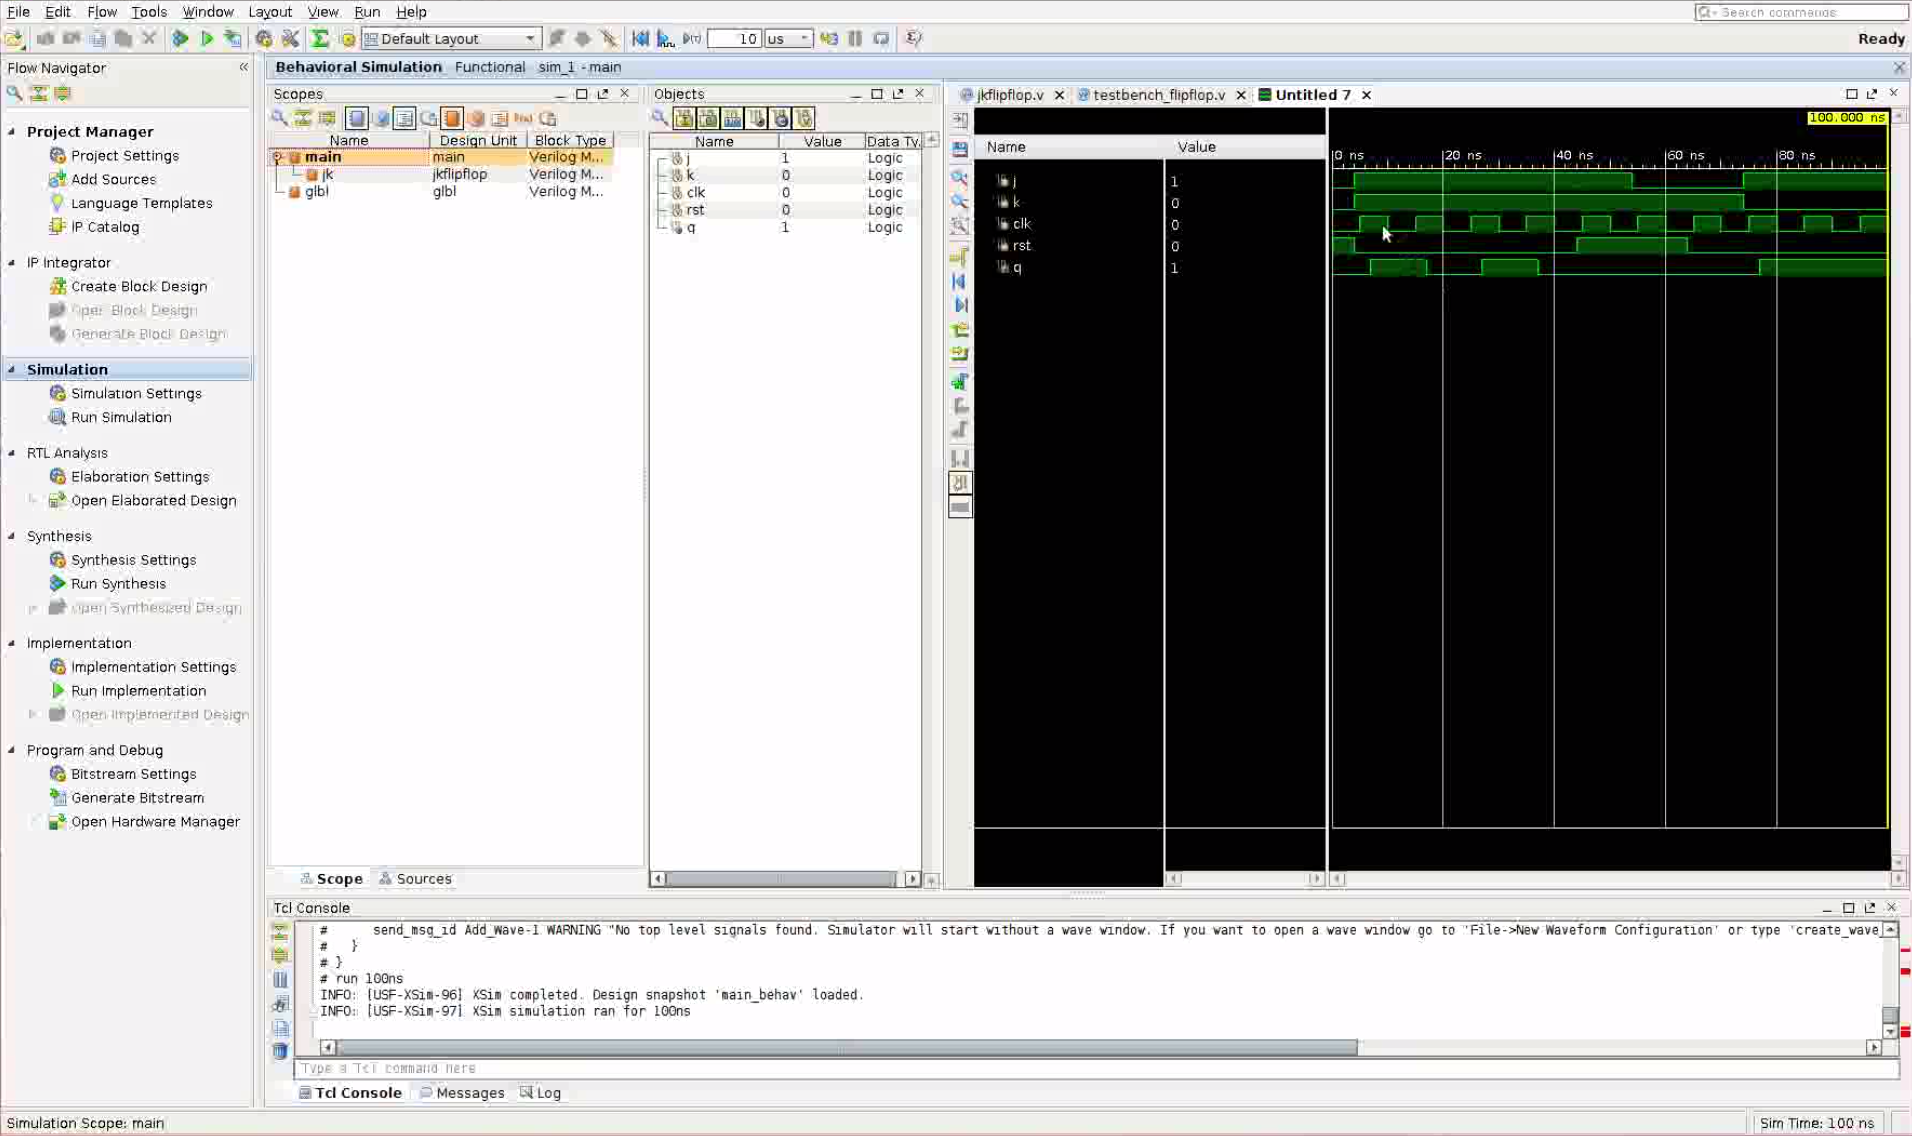
\includegraphics[width=0.8\textwidth, height=0.4\textwidth]{./images/vivado-pro-13.eps}
	\caption{Simulation 1}
	\label{fig:sim_1} 
\end{figure}

\begin{figure}[h!]
	\centering
	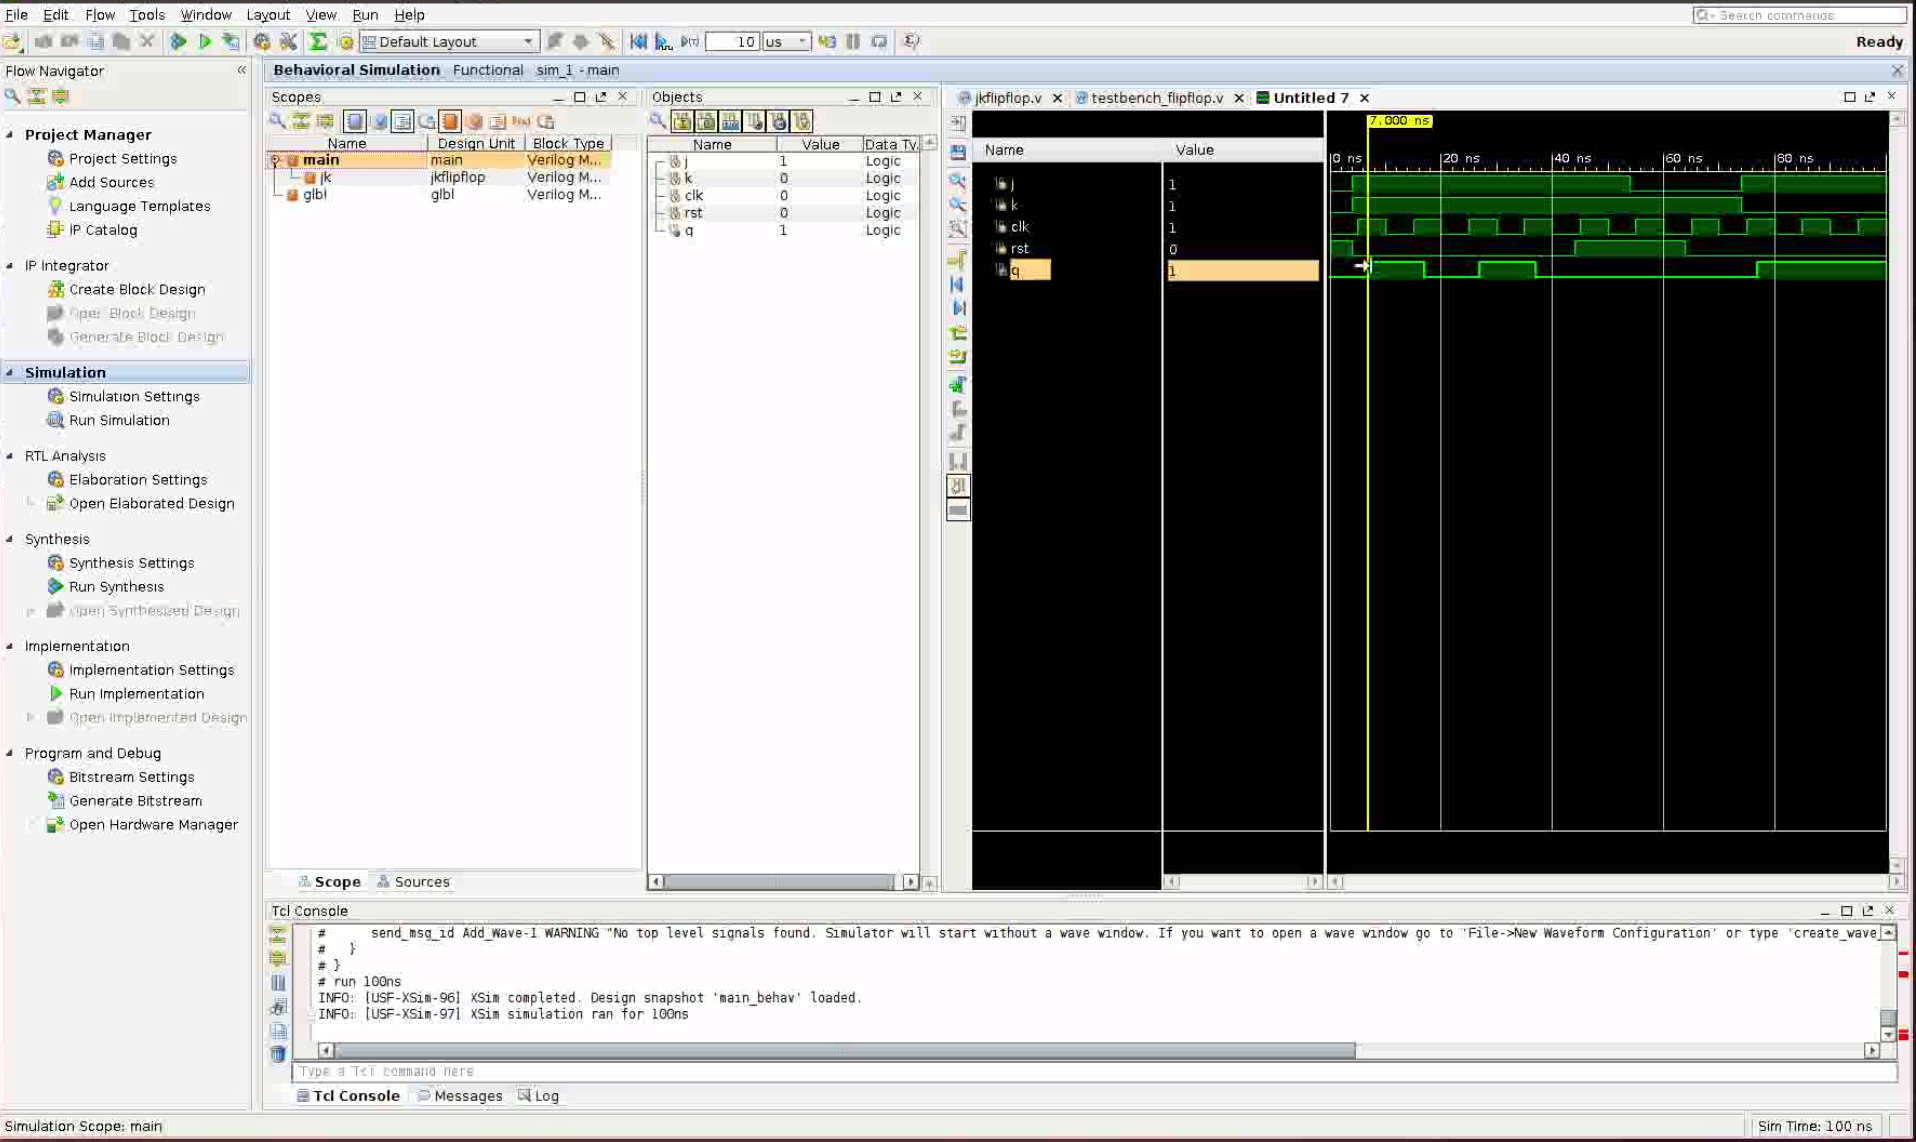
\includegraphics[width=0.8\textwidth, height=0.4\textwidth]{./images/vivado-pro-14.eps}
	\caption{Simulation 2}
	\label{fig:sim_2} 
\end{figure}

\begin{figure}[h!]
	\centering
	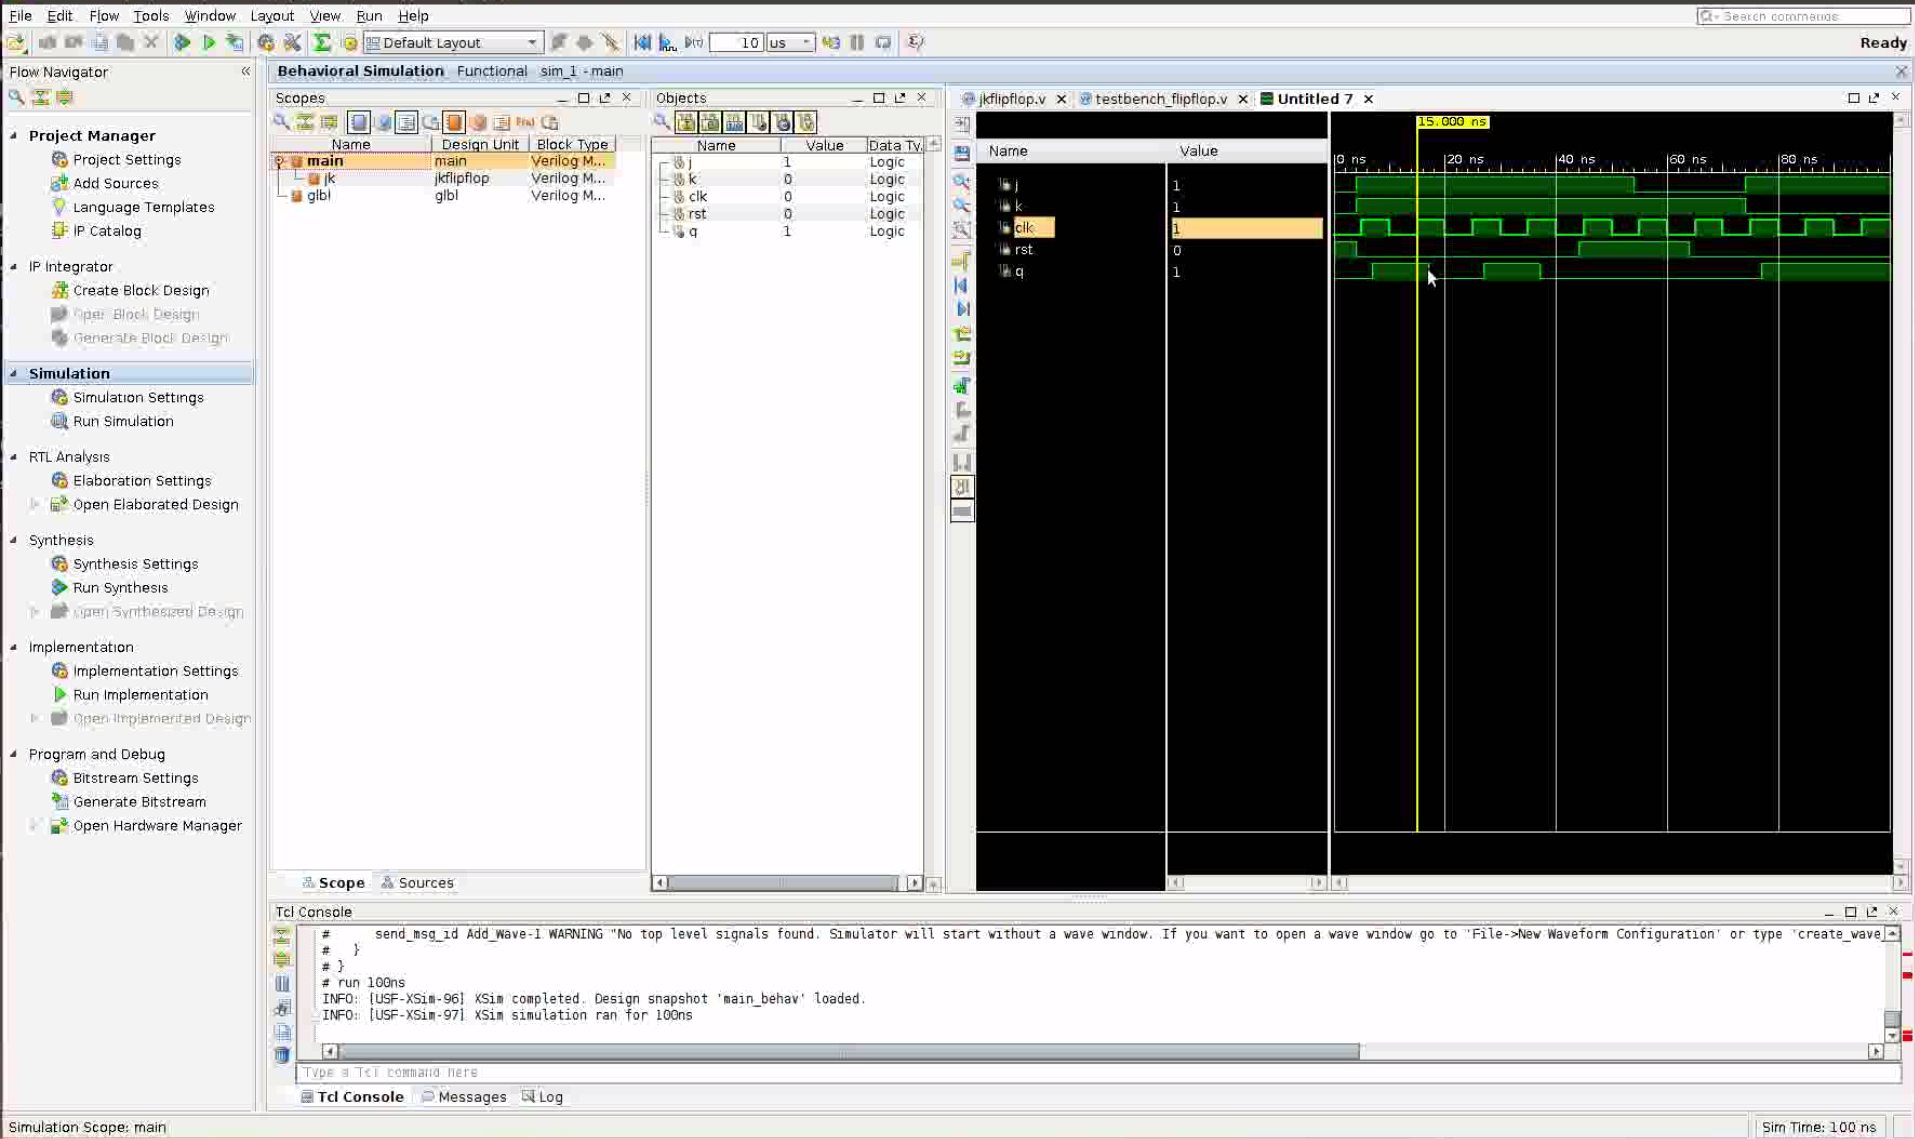
\includegraphics[width=0.8\textwidth, height=0.4\textwidth]{./images/vivado-pro-15.eps}
	\caption{Simulation 3}
	\label{fig:sim_3} 
\end{figure}

\begin{figure}[h!]
	\centering
	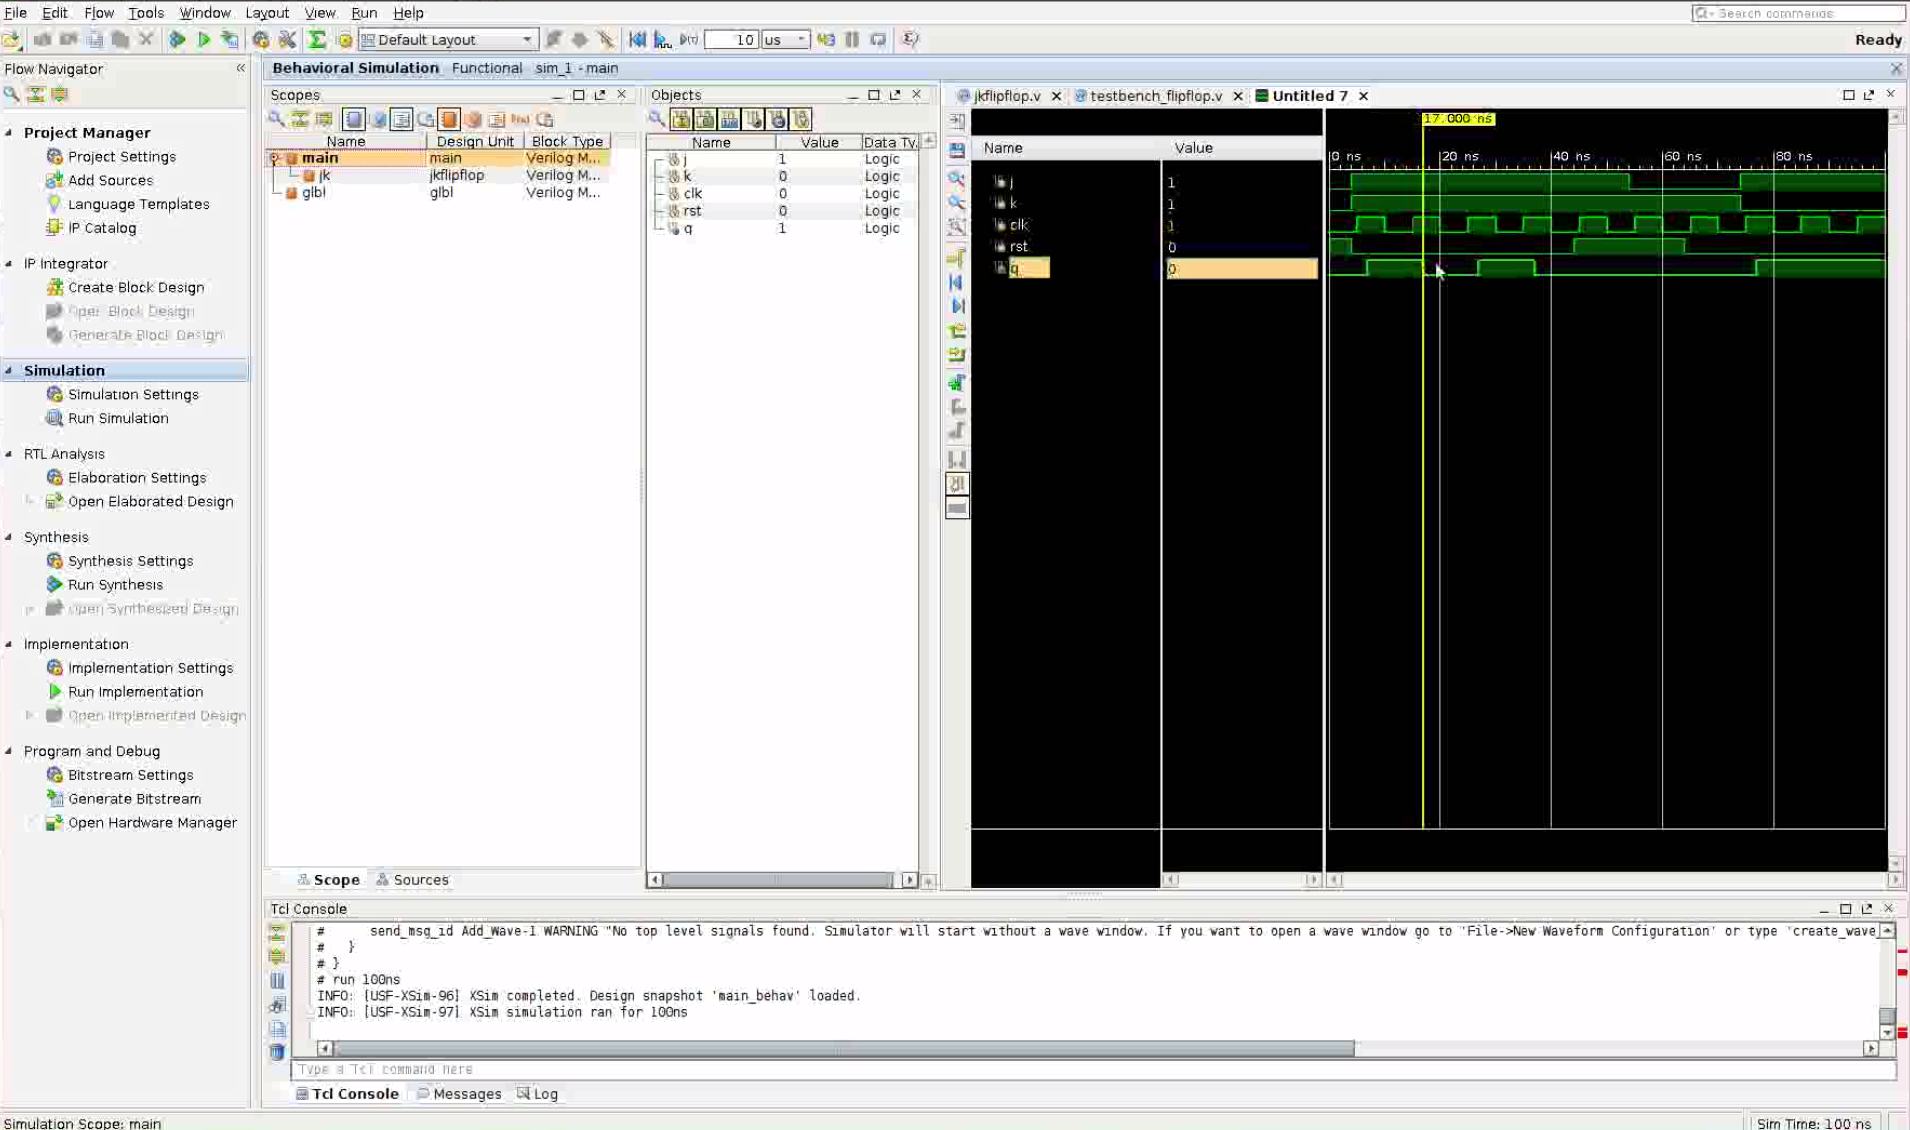
\includegraphics[width=0.8\textwidth, height=0.4\textwidth]{./images/vivado-pro-16.eps}
	\caption{Simulation 4}
	\label{fig:sim_4} 
\end{figure}

\begin{figure}[h!]
	\centering
	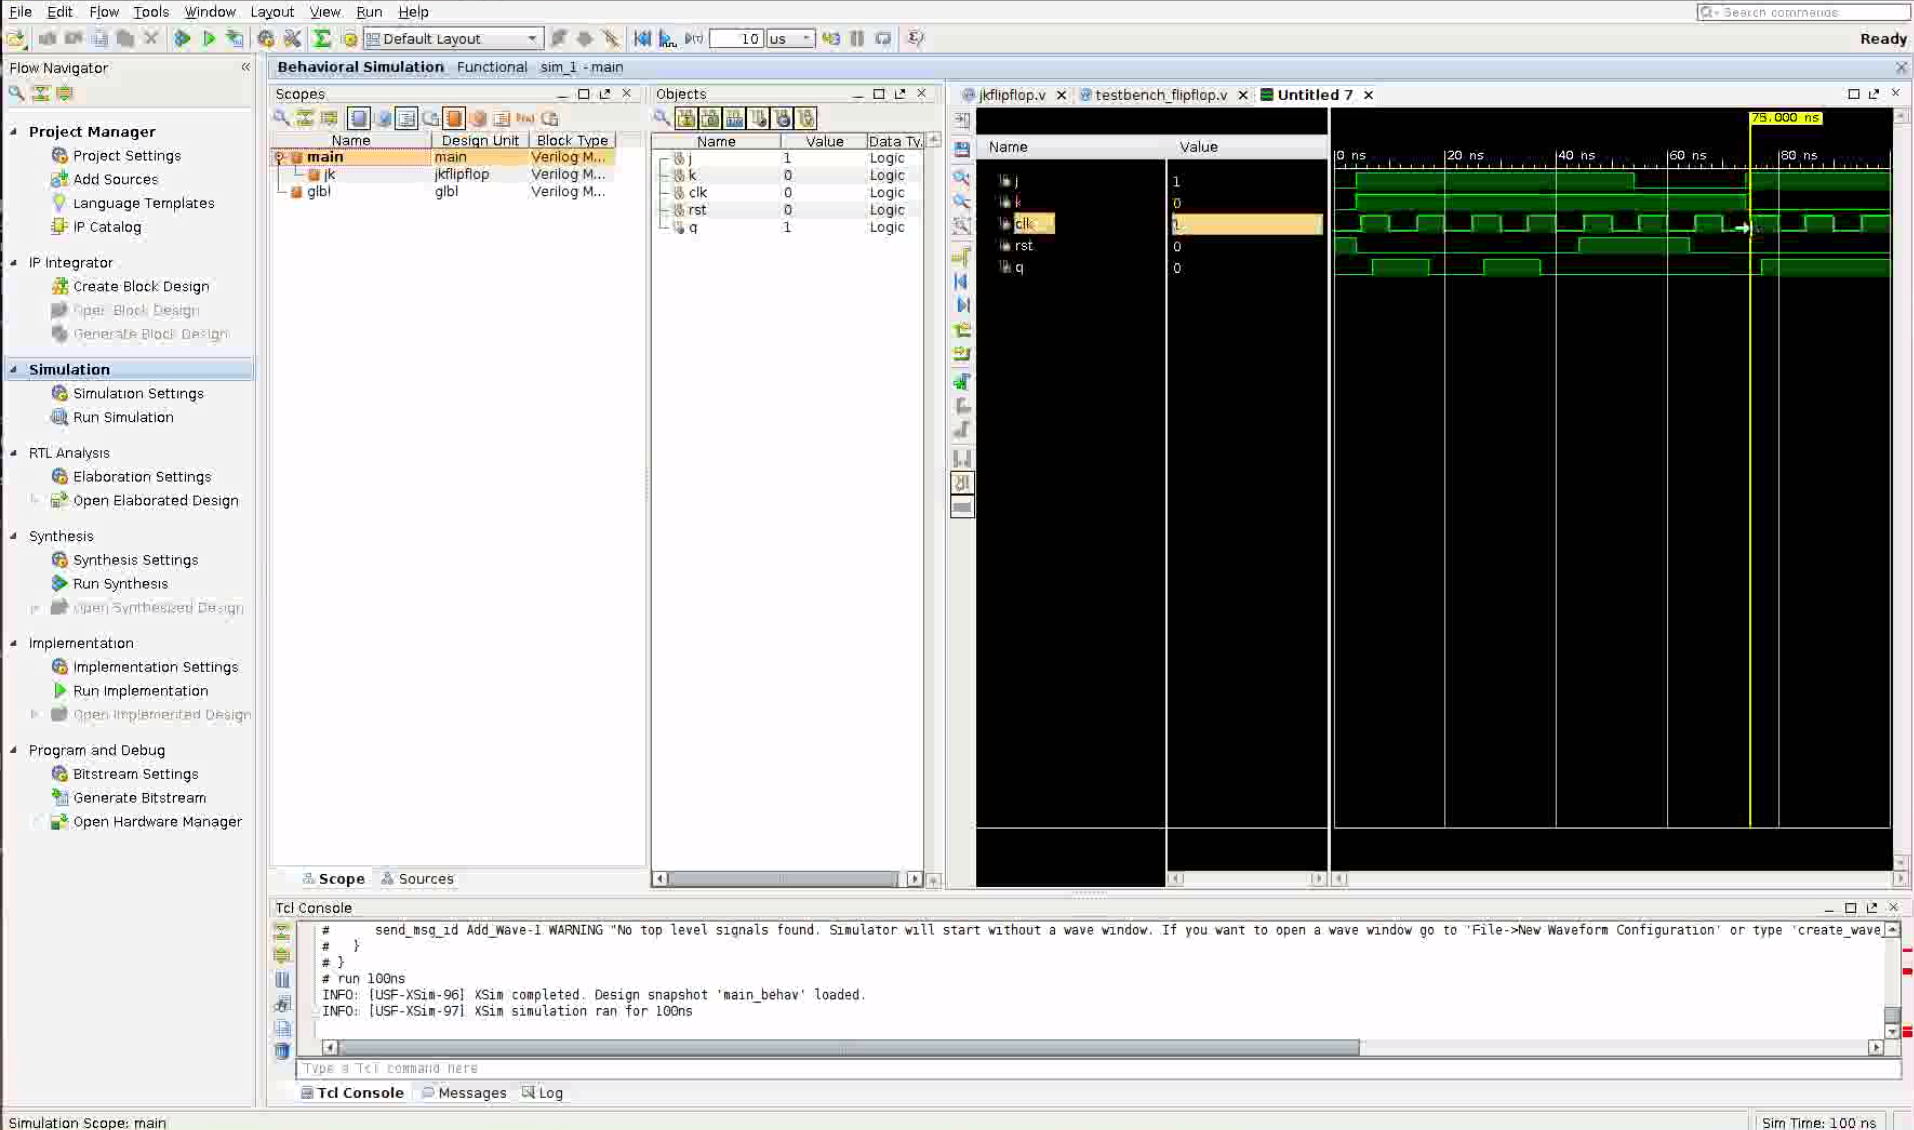
\includegraphics[width=0.8\textwidth, height=0.4\textwidth]{./images/vivado-pro-17.eps}
	\caption{Simulation 5}
	\label{fig:sim_5} 
\end{figure}

\begin{figure}[h!]
	\centering
	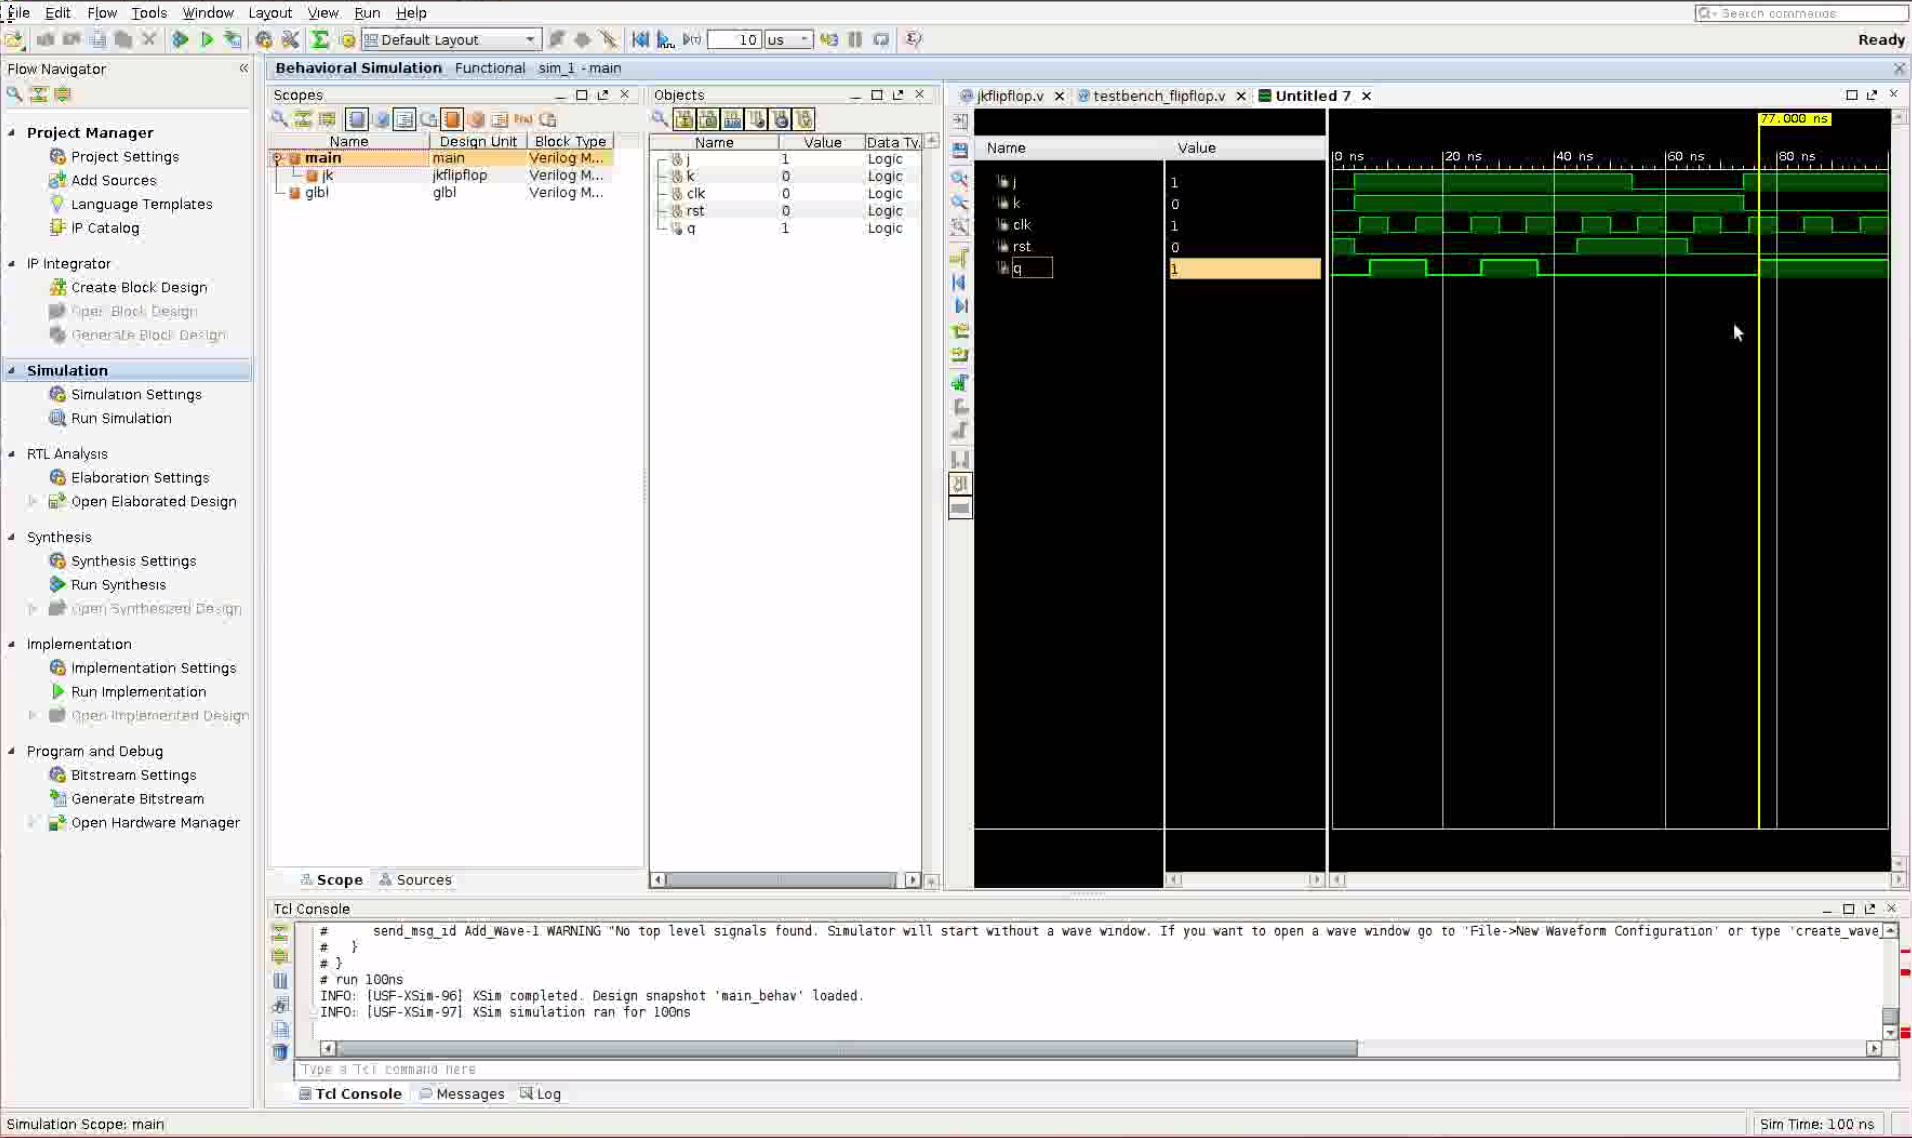
\includegraphics[width=0.8\textwidth, height=0.4\textwidth]{./images/vivado-pro-18.eps}
	\caption{Simulation 6}
	\label{fig:sim_6} 
\end{figure}



\clearpage
\bibliographystyle{unsrtnat}
\bibliography{./refs}

\end{document}

